% This must be in the first 5 lines to tell arXiv to use pdfLaTeX, which is strongly recommended.
\pdfoutput=1
% In particular, the hyperref package requires pdfLaTeX in order to break URLs across lines.

\documentclass[11pt]{article}

% Remove the "review" option to generate the final version.
\usepackage[review]{ACL2023}

% Standard package includes
\usepackage{times}
\usepackage{graphicx}
\usepackage{latexsym}
\usepackage{float}

% For proper rendering and hyphenation of words containing Latin characters (including in bib files)
\usepackage[T1]{fontenc}
% For Vietnamese characters
% \usepackage[T5]{fontenc}
% See https://www.latex-project.org/help/documentation/encguide.pdf for other character sets

% This assumes your files are encoded as UTF8
\usepackage[utf8]{inputenc}

% This is not strictly necessary, and may be commented out.
% However, it will improve the layout of the manuscript,
% and will typically save some space.
\usepackage{microtype}

% This is also not strictly necessary, and may be commented out.
% However, it will improve the aesthetics of text in
% the typewriter font.
\usepackage{inconsolata}

% If the title and author information does not fit in the area allocated, uncomment the following
%
%\setlength\titlebox{<dim>}
%
% and set <dim> to something 5cm or larger.

\title{Building an LLM identifiability challenge}

% Author information can be set in various styles:
% For several authors from the same institution:
\author{Guy Shpigler \and Nir Mezamer \and Yuval Mizrahi \and Yuval Mor \\
        School of Computer Science, Tel-Aviv University\\
        School of Electrical Engineering, Tel-Aviv University \\
        \texttt{\{shpigler,nirmezamer,yuvalmizrahi,yuvalmor3\}@mail.tau.ac.il}}

\begin{document}
{\makeatletter\acl@finalcopytrue
  \maketitle
}
\begin{abstract}

  Natural Language Processing (NLP) has made remarkable progress in recent years across various language-related tasks, and the use of large language models (LLMs) for text generation, summarization, and writing is becoming increasingly widespread.
  However, these advancements have also introduced a new challenge, as distinction between human-generated and machine-generated text becomes less clear.
  With LLMs becoming more sophisticated, they can produce text that closely resembles human-written content in terms of style, syntax, and coherence.
  This blurring of lines poses significant implications for various applications where textual authenticity is crucial, such as in journalism, social media, and online encyclopedia (Wikipedia) where they all serve as primary sources of knowledge for people worldwide. 
  Our research project is designed to help answering this fundamental question:\\
  Given a text, was it generated by a human or by a large language model (LLM)?\\
  To address this question, we first design a pipeline to gather diverse human-generated texts in specific domains (Wikipedia, Reddit posts and comments, newspaper articles).
  By selecting a wide array of sources, we ensure that our dataset captures a broad spectrum of writing styles, topics, and formats. This diversity is crucial for creating a robust challenge.
  Based on these human-texts, we then design a pipeline to collect LLM-based texts mimicking the same diversity and domains as the natural ones. This involves using the large language model Gemini\footnote{\url{https://ai.google.dev/}} to generate texts that replicate the styles and contexts of the human texts, and can be modified to use other LLMs.
  Our goal is to create a dataset where the machine-generated texts are as indistinguishable as possible from the human-generated ones at first glance. 
  Subsequently, the dataset will form the foundational training infrastructure for machine learning models.
\end{abstract}

\section{Introduction}
To address the classification question, we aim to build a robust infrastructure for creating a Neural Network model that, given a text input, can determine whether it was generated by a human or by an LLM. The model's performance will largely depend on the quality of the dataset we build, which will be used for the model's learning process.
The main challenge of our project was to create two text corpora: one of texts generated by humans and the other of texts generated by LLMs. Both corpora need to be representative, diverse, and balanced in size.
We started by building the corpus of human-generated texts. To meet the requirements mentioned above, we chose to extract texts from various sources such as Wikipedia, Reddit (a social network) and newspapers.
To create this text corpus, we wrote python scripts that use open APIs such as Wikipedia API\footnote{\url{https://pypi.org/project/Wikipedia-API/}}, Reddit API\footnote{\url{https://praw.readthedocs.io/en/latest/}}, and Newspaper3k API\footnote{\url{https://newspaper.readthedocs.io/en/latest/}}. From these, we extracted Wikipedia pages, posts and comments from Reddit, and published newspaper articles from the BBC, which together form the corpus of human-generated texts. The topics in each domain were selected using a random mechanism to ensure as much diversity as possible. The pipepline for collecting human-generated texts can be easily extended to other domains and sources.
Simultaneously, to create the dataset of texts generated by LLMs, we used the Gemini API. We hand-crafted several prompts for each domain to achieve the most appropriate one to use when generating texts.
Using the labeled data, we trained a classifier model to distinguish between human-generated and LLM-generated texts. We used a pre-trained BERT model and fine-tuned it on our dataset.

\begin{figure*}[tp]
  \centering
  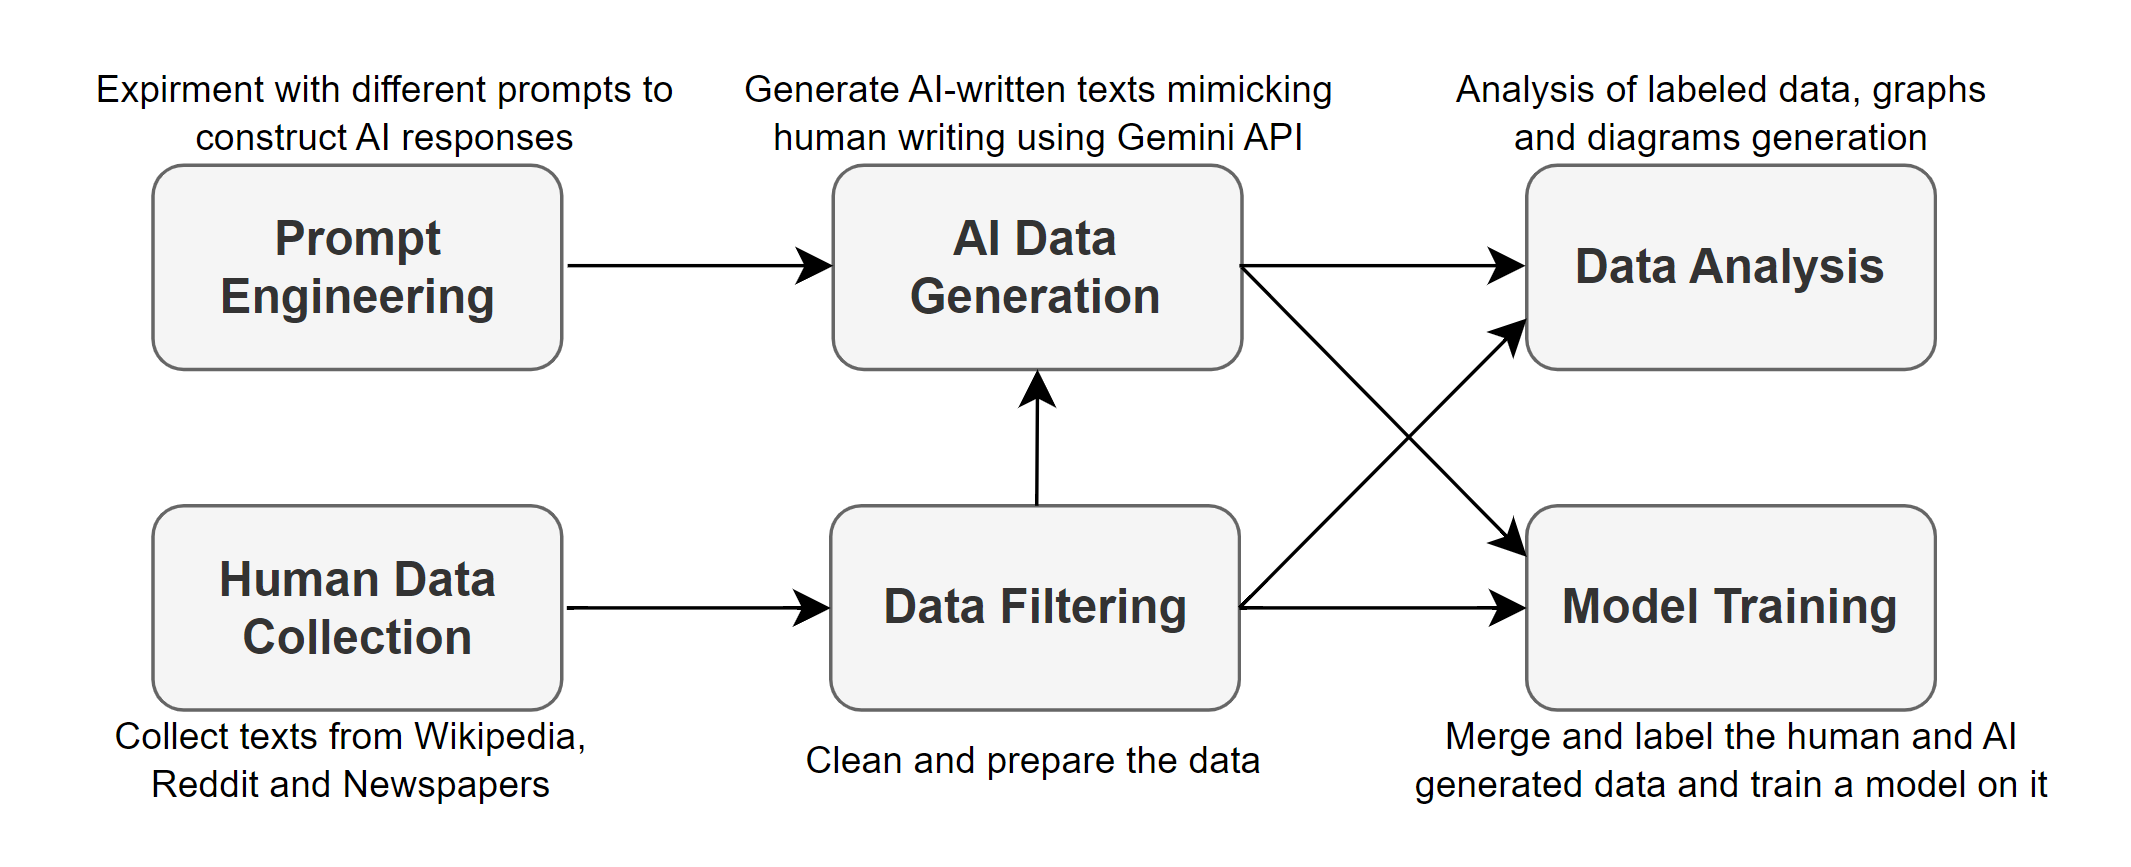
\includegraphics[width=\textwidth]{overview_diagram.png}
  \caption{Project overview diagram}
  \label{fig:pipeline}
\end{figure*}

\section{Related Work}
Our project focuses on assessing the ability to distinguish between texts generated by humans and those generated by machines. Specifically, we aim to create a pipeline to gather dataset that serves as a robust infrastructure for training models to excel in this task.   
In order to perform this task to the best of our ability, we first researched academic papers that were published, addressing the same topic and gained insights regarding the most suitable working method for our project.
In a recent study by \citet{GRiD} published in May 2024 by Qazi, Shiao and Papalexakis, they introduced GRiD (GPT Reddit Dataset), a new collection of texts generated by the Generative Pretrained Transformer (GPT). This dataset is designed to evaluate detection models' performance in identifying responses generated by ChatGPT.
Despite the valuable insights gained from this study, since the dataset was entirely based on a single domain - Reddit, the question arises as to how texts from different domains and with different characteristics will be classified. We will examine this question in this project by constructing a diverse dataset as detailed above. In the following sections, we present our methodology, experimental setup, and results.
For implementing the task of distinguishing between human-generated and machine-generated texts, a model was implemented relying on \citet{BERT}, which describes how to use a pre-trained BERT model and fine-tune it on a dataset. \\ \\

\section{Methodology}
\subsection{Objective}
The main objective of the research is to explore the ability of different language models to distinguish between texts generated by humans and those generated by LLM (Large Language Models).
\subsection{Data Collection}
As mentioned above, the main task was to collect and generate the appropriate data for training the model. At this stage, we needed to collect authentic texts created by humans, texts with the same context generated by LLM, and process the generated data.
During the research, we focused on three main sources of text:\\ Reddit, Wikipedia and Newspaper websites.
\subsubsection{Reddit}
Reddit is a social news aggregation, web content rating, and discussion website. Registered members submit content to the site such as links, text posts, and images, which are then voted up or down by other members. Posts are organized by subject into user-created boards called "subreddits", which cover a variety of topics including news, science, movies, video games, music, books, fitness, food, and image-sharing.\\
Our final dataset contains a collection of posts, where from each post we extracted one comment created by a human and one generated by an LLM.
We gathered the human-written comments using the Reddit API (PRAW), and the AI-generated comments were created using the Gemini API. The goal during the collection process was to create a large, reliable, and diverse dataset. 
To meet those criteria, we initially collected posts with comments from several subreddits, which were chosen randomly from the most popular subreddits list, in order to ensure as much diversity as possible. A total of 10,000 posts were collected.
As mentioned above, for each post we extracted from Reddit, we chose one human-generated comment and one AI-generated comment. To create an AI generated comment for each post, we crafted a prompt which requests the model to create a suitable comment for the post. The prompt included the following fields: post's title, post's content, post's subreddit, and 4 of the post's comments. The comment which was used as the human-generated comment for the dataset was not included in the prompt. In this way, we ensure that our dataset is reliable and challenging for learning, as the comment generated by the LLM is strongly based on texts created by humans.
Using 4 random comments for the prompt didn't yield good results, since most of the comments did not appear to match human text. For example, comments containing a URL link, such as a link to an image, "[REMOVED]" comments indicating that a user's comment was deleted, unusual characters like emojis, very short comments like "great" or "ok", etc. Additionally, some comments contained offensive or racist information and tone, which can not be used as part of the prompt (blocked by the Gemini API).
To overcome the mentioned problem, a cleaning and preprocess procedure of the dataset was added. In the first stage, all non-text characters were removed from the comment. In the second stage, the list of comments in each post was sorted in such a way that the top comments in each post would be the best according to the parameters mentioned above. Of course, there is no direct way to do this, so we relied on external sources and created a weighting function that gives high scores to authentic comments and low scores to comments that are not authentic or offensive. Only around 70\% of the posts were used in the final dataset, as the rest were filtered out due to the reasons mentioned above.
This process proved successful, where the final dataset we created was in the format of a post with two comments: one is taken from the top 5 human comments, and the other is the comment generated by Gemini.
\subsubsection{Wikipedia}
Wikipedia is a free online encyclopedia, created and edited by volunteers around the world and hosted by the Wikimedia Foundation.
The website has a free API, which was used to extract articles from Wikipedia. Only articles which has an attribute of "summary" were extracted - a total of 4000 articles. Half of the articles comprised the human generated part of the dataset. In addition, only the titles of the other half were inserted into an hand-crafted prompt, which in turn was fed to the Gemini model, to generate 2000 AI generated wikipedia style summaries. Many expirments were made in order to craft the most suitable prompt, and also to determine the best approach. At first the prompt didn't include a specific title, and the request was to generate a random article summary in a Wikipedia style. That attempt didn't work because the model repeated itself quite a lot. The second attempt was to give the model the title and body of the article (without the summary), and ask it to generate the summary. That attempt worked too well, generating a summary which is very similiar to the real summary - probably because the model was trained on that data. The final attempt was to give the model the title of the article, and it worked quite well. The code can be easily scaled up to generate more summaries, both human and AI generated - limited by the number of articles in the English Wikipedia, which is around 6 million.
\subsubsection{Newspaper}
First, we used the Newspaper3k API to obtain articles published recently on the BBC website. An attempt was made to obtain articles from various different news sites (CNN, Fox News, NYT…) but most sites blocked the API calls after a small amount of tries, requiring a payment for extensive API usage. We then crafted another prompt and sent it to Gemini, including the original article (title and content). The prompt included a request to recreate the article, keeping the generated content closely aligned with the given text, while emphasizing to the model to "write originally and use its own words". As opposed to Wikipedia, the model was not trained on the BBC articles, so the generated articles were more diverse and less similar to the original articles. Some of the articles extracted by the API were extremely short (breaking news headlines) and unsuitable for inclusion in the dataset. By setting a length requirement, these shorter articles were filtered, which yielded better results. A total of 300 articles were collected, half were used to create the AI generated part of the dataset, and the other half were used as the human generated.
\subsubsection{Conclusion of the Data Collection}
In accordance with the aforementioned descriptions, three distinct techniques and methods were employed for generating the AI texts. This multifaceted approach not only enhances data diversity but also elevates the overall quality of the dataset. The resulting dataset comprises 18,000 labeled samples, evenly split between human-generated and AI-generated texts. This balanced and diverse dataset is suitable for training models to differentiate between human and AI-generated texts. The dataset's diversity is further exemplified by the various sources from which the data was collected, as well as the different text styles, formats, and lengths.
\subsection{Model}
To further evaluate the usability of our dataset, we employed a BERT classifier, a transformer model developed and pre-trained by Google. This model is specifically designed for natural language processing tasks and provides a robust framework for text classification.
Our dataset consists of two columns: "data" and "label". The "data" column includes the textual data, while the "label" column contains binary labels indicating the origin of the text (0 for human-generated and 1 for AI-generated). To adapt BERT for our classification task, we added a fully connected layer with a single output neuron. By applying the sigmoid activation function to this output, we obtained the probability of each text being human or AI-generated.
We utilized the Binary Cross Entropy Loss (BCELoss) as our loss function, which is suitable for binary classification tasks. The model was trained for 15 epochs with a batch size of 32, using the AdamW optimizer with a learning rate of 2e-5. The training and validation accuracy were monitored to evaluate the model's performance. The training was conducted on Google Colab\footnote{\url{https://colab.research.google.com/}}, using the T4 GPU provided by Google.\\\\
All of the code, including relevant graphs and documentation can be found in our Github repository\footnote{\url{https://github.com/nirmezamer/NLP_final_project.git}}.

\section{Experiments}
\subsection{Dataset Analysis}
In our analysis, we utilized several classic techniques to examine and compare AI-generated and human-generated texts across different datasets. We began by visualizing the distribution of the number of words, characters, unique words, and sentences using histograms. These visualizations reveal a clear distinction between human and AI-generated texts.\\
\begin{figure}[H]
  \centering
  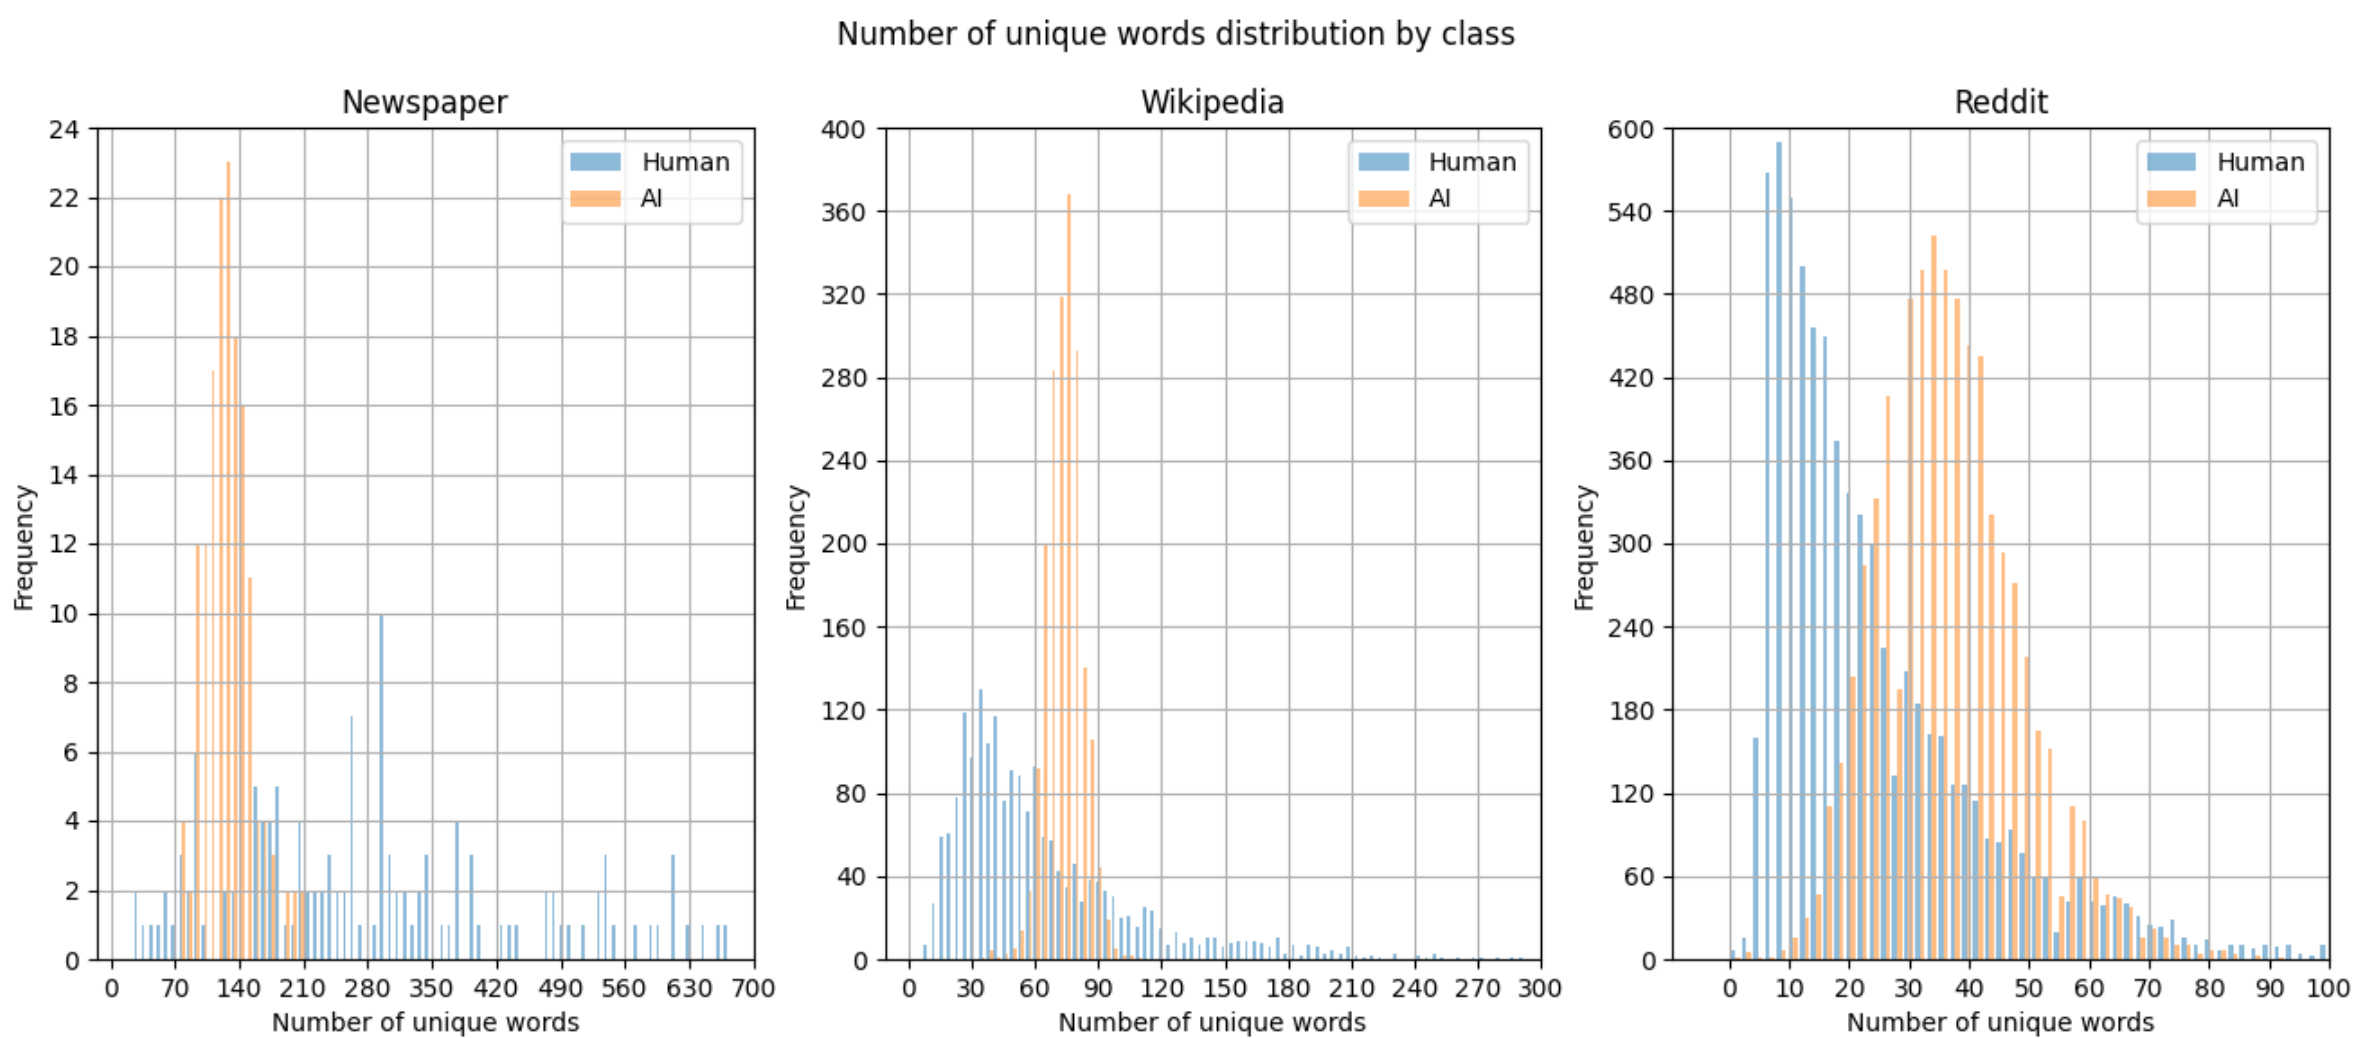
\includegraphics[width=\linewidth]{unique_words.png}
  \caption{Histograms of unique words in human and AI-generated texts}
  \label{fig:unique_words}
\end{figure}

As seen in figure \ref{fig:unique_words}, the histograms of unique words in human and AI-generated texts (more histograms can be found in the Github repository) demonstrate notable differences.
In the Wikipedia and newspaper datasets, human-generated texts exhibit a broader distribution in terms of the number of words, characters, unique words, and sentences compared to AI-generated texts. This indicates that human writing in these contexts tends to vary more in length and complexity. Conversely, in the Reddit comments dataset, AI-generated texts show a wider distribution than human-generated texts. This can be attributed to the informal and typically shorter nature of Reddit comments, which contrasts with the more formal and extended format of Wikipedia and newspaper articles.

\begin{figure}[H]
  \centering
  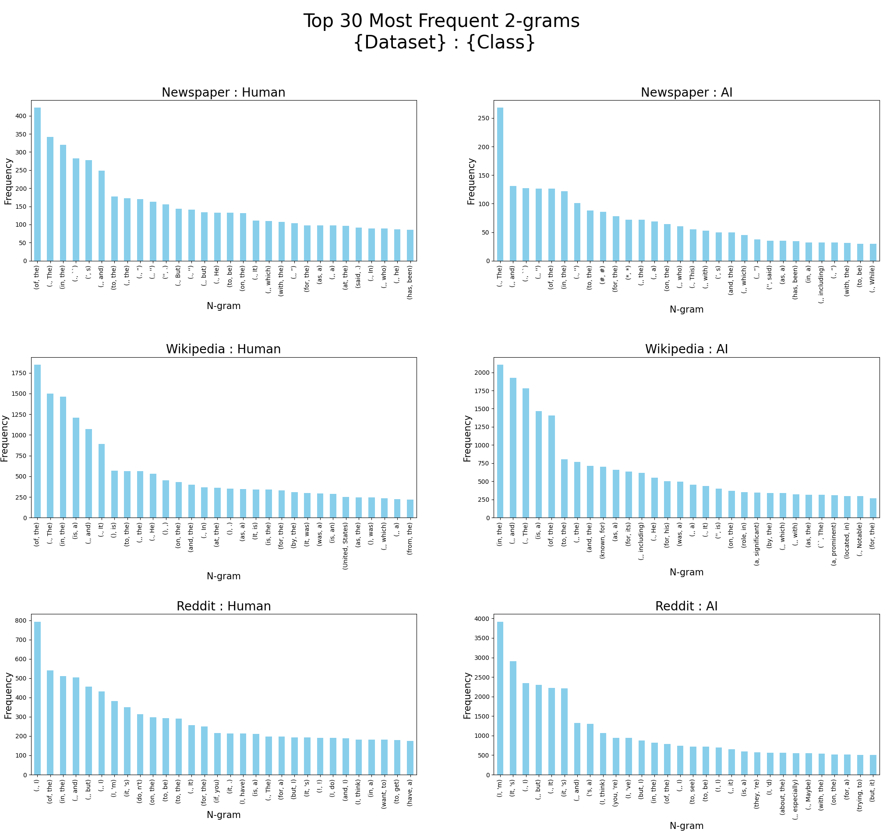
\includegraphics[width=\linewidth]{2_grams.png}
  \caption{2-gram analysis of human and AI-generated texts}
  \label{fig:n-grams}
\end{figure}
Furthermore, we analyzed the most frequent n-grams (combinations of words) within the datasets, as seen in figure \ref{fig:n-grams} (more n-grams analysis can be found in the Github repository). This analysis highlights significant differences between human and AI-generated n-grams. Human-generated texts tend to have n-grams that are used more frequently than those in AI-generated texts. This suggests that human writing often relies on common phrases and constructs, while AI-generated texts may exhibit a more diverse range of expressions. The n-gram analysis thus provides insights into the distinctive patterns of language use between human and AI texts.

\begin{figure}[H]
  \centering
  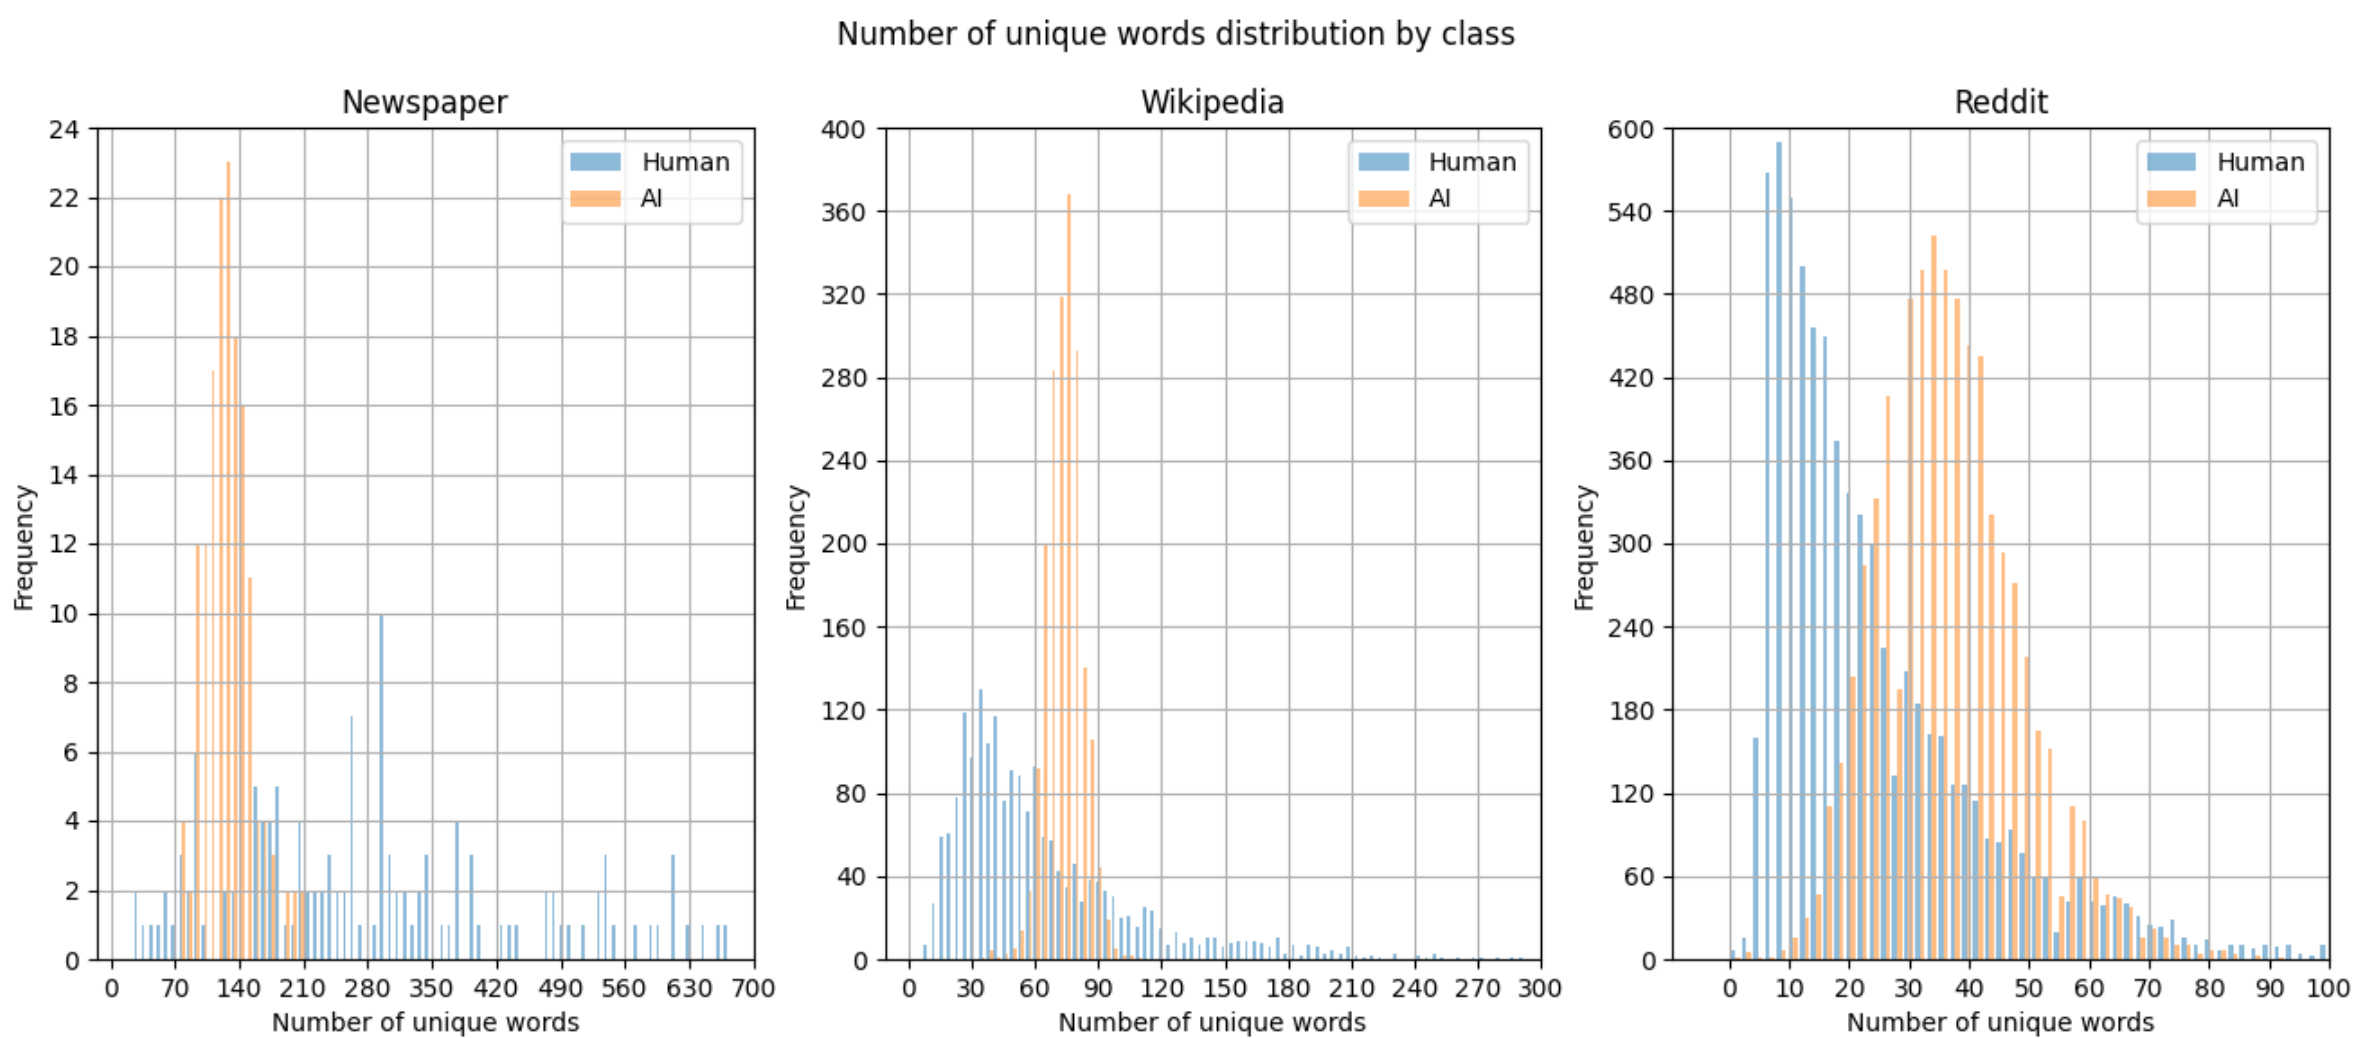
\includegraphics[width=\linewidth]{unique_words.png}
  \caption{Word clouds of human and AI-generated texts}
  \label{fig:word_clouds}
\end{figure}
The word clouds generated from the datasets further illustrate these differences, as shown in figure \ref{fig:word_clouds}. In word clouds, the size of a word corresponds to its frequency in the text. Human-generated texts typically result in larger word clouds, reflecting a higher repetition of certain words or phrases. On the other hand, AI-generated texts produce more diverse word clouds, indicating a broader vocabulary and varied word usage. This diversity in AI-generated word clouds underscores the algorithmic attempts to create varied and less repetitive content.

Overall, our analysis reveals that human-generated texts are more varied and nuanced, especially in formal contexts like Wikipedia and newspapers. In contrast, AI-generated texts, while potentially more diverse in vocabulary, tend to be more consistent in length and structure, particularly in informal contexts like Reddit comments. These findings highlight the intrinsic differences in content generation between humans and AI, offering valuable insights for understanding and improving AI text generation technologies.
\\
\\
\subsection{Model Evaluation}

\begin{figure}[H]
  \centering
  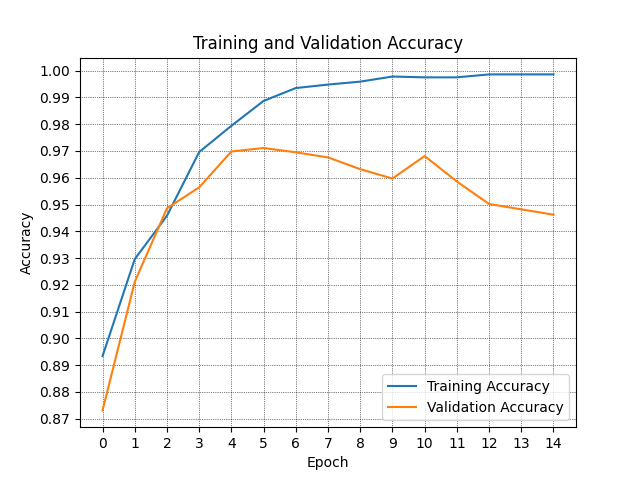
\includegraphics[width=\linewidth]{accuracy.png}
  \caption{Training and validation accuracy over 15 epochs}
  \label{fig:example}
\end{figure}

The accompanying graph illustrates the training and validation accuracy over the epochs.
From the graph, it is evident that the model effectively distinguishes between human and AI-generated texts. The training accuracy rapidly increases, approaching near-perfect performance within a few epochs. However, the validation accuracy exhibits a different trend, initially improving but then fluctuating and showing signs of decline as the epochs progress. This divergence between training and validation accuracy indicates overfitting, a common issue when the model learns to perform exceptionally well on the training data but fails to generalize to unseen data.
The overfitting observed here is likely due to the relatively small size of our dataset. With limited data, the model can easily memorize the training examples, leading to high training accuracy but poor generalization. This emphasizes the need for larger and more diverse datasets to train models that can generalize well to new, unseen texts.
In conclusion, while the BERT classifier demonstrates high performance on the training data, the validation results highlight the importance of addressing overfitting. This analysis underscores the dataset's utility in distinguishing between human and AI-generated texts but also points to the need for further data augmentation and regularization techniques to improve generalization.

\section{Discussion and Conclusion}
In our comprehensive study, we focused on the ability to answer the question of the origin of a given text. Ultimately, a deep learning model will answer this question by receiving a text as input and providing a classification response as output. The classification question is difficult and perhaps impossible for humans due to the rapid development of LLMs, this research demonstrates a pipeline which can be used to train a model to solve this problem. By creating a diverse, large, and balanced dataset, high performance and very high accuracy rates can be achieved.
The essence of the research is to create a dataset that is as close as possible to the real world, where the texts generated by the LLM are indistinguishable from the human-generated texts. Further improvement of the dataset can be achived by utilizing more sources and domains, using multiple LLMs to generate the AI texts and even applying a sort of a MixUp augmentation technique, where a random human text is mixed with a random AI text. This will increase the diversity of the dataset.
Over time, of course, LLMs will improve significantly and rapidly, making the classification question of whether a text was created by a human or an LLM even more challenging. However, our research provides hope and indicates a close connection between the construction of the dataset intended for training the model and the ability of a deep learning model to notice differences, even those not visible to the eye, between different types of texts.

\bibliography{custom}
\bibliographystyle{plainnat}

\appendix

\section{Example Appendix}
\label{sec:appendix}

This is a section in the appendix.

\end{document}